\chapter{Prestazioni}
\label{prestazioni}

In questo capitolo viene mostrato l'esito in termini di performance delle modifiche apportate. Le prestazioni sono state misurate tramite uno script ereditato dal lavoro precedente sulla libreria FIDO opportunamente modificato per lo scopo. L'esito delle misurazioni è in linea con quanto già constatato precedentemente. 

\section{Raccolta dei dati}
\label{raccolta_dati}

Per prendere le misurazioni relative alle performance è stato utilizzato un calcolatore con sistema operativo Fedora 36, dotato di CPU Intel i5-8250U e un autenticatore CTAP2 emulato virtualmente tramite il backend UDP descritto nel capitolo precedente \ref{testing}. Grazie all'emulatore è stato possibile inibire la mediazione dell'utente richiesta, sia in fase di creazione delle credenziali che di autenticazione. Così facendo il dato ottenuto risulta deterministico.

I tempi di esecuzioni sono stati presi tramite l'ausilio della libreria Python \verb*|timeit|, che prende come parametro una funzione e il numero di volte che deve essere eseguita, restituendo il tempo di esecuzione. I metodi provati sono stati quelli descritti nei capitoli precedenti:

Per la fase di creazione delle credenziali
\begin{itemize}
	\item \verb*|register_begin()|
	\item \verb*|make_credential()|
	\item \verb*|register_complete()|
\end{itemize}
E per la fase di autenticazione
\begin{itemize}
	\item \verb*|authenticate_begin()|
	\item \verb*|get_assertion()|
	\item \verb*|authenticate_complete()|
\end{itemize}

Per ogni livello di sicurezza \emph{n} stabilito, i test sono stati ripetuti con un livello di sicurezza in fase di \textbf{autenticazione} \emph{k} tale che: $k \in [1, n]$. Per diminuire la variabilità dei dati i tempi del metodo \verb*|get_assertion()| sono stati presi sulla base della media di dieci iterazioni. La fase di creazione è stata, invece, ripetuta solamente una volta.

\section{Valutazione dei dati}
\label{valutazione}

I dati nel grafico sono relativi sia alle fasi di creazione che di autenticazione, cioè al tempo totale misurato.
\begin{center}
	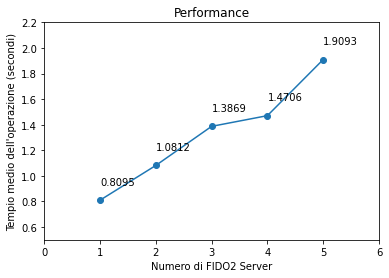
\includegraphics[scale=0.65]{figures/test_results}
\end{center}

Come si può notare dal grafico all'aumentare del livello di sicurezza, e quindi del numero di FIDO Server, il tempo totale cresce di circa 30 \emph{ms}. Con 5 FIDO Server il tempo di esecuzione totale è più che raddoppiato. Si nota un'anomalia in corrispondenza di quattro FIDO Server ma il trend rimane comunque crescente.

I tempi per la fase di creazione delle credenziali riportano un risultato simile: un incremento di circa 20 \emph{ms} per ogni FIDO Server aggiuntivo. Anche qui è presente la stessa anomalia citata sopra. 
\begin{center}
	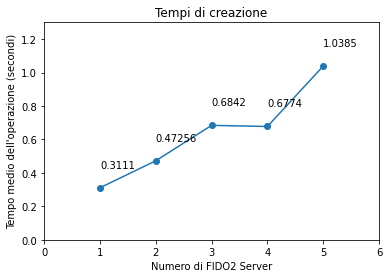
\includegraphics[scale=0.65]{figures/creation_results}
\end{center}

I tempi della fase di autenticazione sono cresciuti più lentamente all'aumentare del livello di sicurezza richiesto in fase di autenticazione. In legenda sono indicati i FIDO Server attivi volta per volta e quindi il livello di sicurezza richiesto in fase di creazione delle credenziali. I punti sul grafico rappresentano il tempo necessario a completare l'operazione per ogni security level in fase di autenticazione, da \emph{1} a \emph{n}.
\begin{center}
	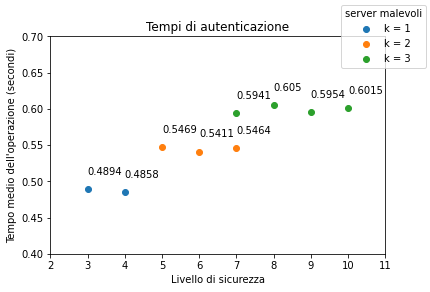
\includegraphics[scale=0.65]{figures/auth_results}
\end{center}

Occorre precisare che le misurazioni effettuate sono assolutamente ottimistiche sia per quanto riguarda la latenza con i FIDO Server, operanti localmente, che per quella con l'autenticatore, emulato virtualmente. Inoltre, non tengono conto dell'interazione umana richiesta e dell'utilizzo di un Web Browser con le penalizzazioni che ne conseguono. 

Si può quindi concludere dai dati raccolti che l'incremento di tempo richiesto dall'operazione con una combinazione di \emph{k} e \emph{n} adeguata è di pochi \emph{ms} in più a fronte di una \emph{survivability} migliore. Per numeri di FIDO Server alti l'operazione richiede, però, un tempo doppio rispetto al normale, costituendo una penalizzazione di fatto non trascurabile.
